\documentclass[conference]{IEEEtran}
\IEEEoverridecommandlockouts
% The preceding line is only needed to identify funding in the first footnote. If that is unneeded, please comment it out.
\usepackage{cite}
\usepackage{amsmath,amssymb,amsfonts}
\usepackage{algorithmic}
\usepackage{graphicx}
\usepackage{textcomp}
\usepackage{xcolor}
\usepackage{float}
\def\BibTeX{{\rm B\kern-.05em{\sc i\kern-.025em b}\kern-.08em
    T\kern-.1667em\lower.7ex\hbox{E}\kern-.125emX}}
\begin{document}

\title{Oops I Did It A-GAN\\
}

\author{\IEEEauthorblockN{Michael Watts}
\IEEEauthorblockA{\textit{Computer Science Department} \\
\textit{Southern Methodist University}\\
Dallas, Texas \\
mcwatts@smu.edu}
\and
\IEEEauthorblockN{2\textsuperscript{nd} Given Name Surname}
\IEEEauthorblockA{\textit{dept. name of organization (of Aff.)} \\
\textit{name of organization (of Aff.)}\\
City, Country \\
email address or ORCID}
\and
\IEEEauthorblockN{Siddhika Ghaisas}
\IEEEauthorblockA{\textit{Computer Science Department} \\
\textit{Southern Methodist University}\\
Dallas, Texas \\
sghaisas@smu.edu}
}

\maketitle

\begin{abstract}
Lorem Ipsum
\end{abstract}

\begin{IEEEkeywords}
component, formatting, style, styling, insert
\end{IEEEkeywords}

\section{Introduction}

Generative Adversarial Networks capitalize on the competition between a generative and a discriminative model to guide the generative model towards being able to create samples from its model distribution that are tantamount to samples from the original data distribution. Using this technique navigates around the usual problems in deep generative models of trying to model a probability distribution with intractable computations [1]. This adversarial framework has enabled GANs to achieve impressive results in the realm of image generation [cite high fidelity gan paper]. 
\newline \indent GANs, however, aren’t perfect. The training process suffers from problems including non-convergence, mode collapse, and vanishing generator gradients [cite medium article]. In order to improve the problem of the generator’s gradient vanishing given a discriminator that identifies fake samples with high confidence, Goodfellow suggested a heuristic-based generator loss function in which the generator maximize the expectation of the discriminator being mistaken, instead of minimizing the expectation of the discriminator being correct [2]. Goodfellow claims that this new loss function provides the generator with a better loss landscape and stronger gradient to be calculated. 
\newline \indent In our work, we propose exploiting the strengths of the gradient landscape of both the original loss function and the heuristic-based loss function to help solve the vanishing gradient problems. Our method was to train a GAN on CIFAR image data in which the loss function switches from maximizing the log probability of the discriminator being mistaken to minimizing the log probability of the discriminator being correct at various points in the training process. INSERT MAIN RESULTS AND CONCLUSIONS HERE. 

%Main results & conclusions
%Fill in later
%Paper organization
%Paper has more GAN background, methodology, results, and analysis sections


\section{Generative Adversarial Networks}
\subsection{A Zero Sum Game}
In its simplest expression, a Generative Adversarial Network is structured as a zero-sum game between two players, the generator and the discriminator. The two players of a GAN are represented by two cost functions defined in terms of their parameters. This game plays out in two scenarios. In one scenario, training examples from observed variables, x, are randomly sampled and used as input for the first player, the discriminator. The discriminator is represented by the function D. The goal of the discriminator is to output the probability that its input is real (sampled from the actual data distribution) rather than artificial (sampled from the generator model distribution), under the assumption that half of the inputs it is given are real and half are artificial. In the other scenario, the generator creates samples G(z) from randomly sampled inputs of the model's latent variables, z, and feeds these samples as input to the discriminator.
\newlabel \indent Given that the artificial samples have a label of 0, then the goal of the discriminator is to make D(G(z)) approach 0,  while the goal of the generator is to make the same quantity approach 1[2]. In other words, the discriminator is attempting to maximize, and the generator is attempting to minimize, how often the discriminator correctly identifies a generated sample as artificial. Since each player's objective is inextricably linked to the other player's objective, without yielding control over the other player's parameters, GANs are typically referred to as a zero-sum game as opposed to as an optimization problem [2].

\subsection{The Generator Loss Function}
\indent The generator creates samples that come from the same distribution as the training data. The generator is defined by a function $G$ that takes z as input and uses $\theta^{(G)}$ as parameters. It wishes to minimize $J(G) (\theta^{(D)}, \theta^{(G)})$ and must do so while only controlling $\theta^{(G)}.$The cost function of generator that achieves this objective can be expressed as \newline\newline
$J(G) (\theta^{(D)}, \theta^{(G)}) = min E_{x \leftarrow g(z)} [ log(1-D(x))]$[2]
\subsection{The Discriminator Loss Function}
\indent The discriminator examines the input samples to determine whether they are real or artificial. It wishes to minimize $J(D)(\theta^{(D)},\theta^{(G)})$ and must do so while controlling only $\theta^{(D)}$.The cost function of discriminator can be expressed as\newline\newline
$J(D) (\theta^{(D)}, \theta^{(G)}) = max E_{x\leftarrow P_{data}} [log D(x_{real})] + E_{x\leftarrow g(z)} [log (1-D(x_{fake}))]$ [2]

\subsection{The Vanishing Gradient Problem}
\indent In the zero sum game previously described, the identical value that the discriminator is trying to minimize and the generator is trying to maximize is a cross entropy value. As the model is early on in its training, the generator will not be very good at creating its artificial samples. However, whenever the discriminator correctly identifies a generated sample as artificial, this causes the generator's gradient to vanish, making it slower at, and less capable of, learning well in the early stages of training. This makes the generator's loss function less than ideal when used in practice.

\subsection{Heuristic, Non-Saturating Game}
The alternative heuristic approach to the generator's loss function proposed in [1] is described as a non-saturating game that aims to avoid this diminishing gradient problem. Rather than training the generator to minimize the log-probability of the discriminator being correct, it is proposed to train G to maximize the log-probability of the discriminator being mistaken. Thus, the target of the cross entropy equation in the generator's loss function is reversed. The resultant generator loss function looks like this: 

\newline INSERT IMAGE HERE
\newline

\section{Methodology}
\subsection{Gradient Landscape Intuition}

\subsection{Derivation of the Loss Function}
Before we begin training our network, it is necessary for us to derive an expression for Goodfellow's original loss function which we can use in our network. To do this, we first need to understand two mathematical identities for expectation functions. It has been shown that: 
\begin{align*}
&E_{s \leftarrow q(s|x)}[F(\alpha)] = \sum_{\forall i} q(s|x^i) * f(x^i) \\
&E_{s \leftarrow q(s|x)}[log(F(\alpha))] = \sum_{\forall i} q(s|x^i) * log(f(x^i))
\end{align*} \cite{b4}
\indent In Goodfellow's original work, he derived that the original loss function for the generator was:
\begin{align*}
    \min_g E_{x \leftarrow g(\zeta)}[log(1-d(x_{f}))]
\end{align*}
Wherein $x_{f}$ represents a generated data point, g($\zeta$) represents the generator network output, and d($x_f$) represents the discriminator output. The goal of this loss function was to minimize when the discriminator is correct. While this was the derived loss function, the actual loss function used as heuristic was: 
\begin{align*}
    \max_g E_{x \leftarrow g(\zeta)}[log(d(x_{f}))]
\end{align*}
This method attempts to maximize when the discriminator is incorrect. Using our mathematical identities of expectation functions, we can see that this new loss heuristic function is the equivalent of the Binary Cross Entropy (BCE) of $d(x_f)$ and it's label (in this case represented as 0). 
\begin{align*}
    \max_g E_{x \leftarrow g(\zeta)}[log(d(x_{f}))] = BCE(0, d(x_f))
\end{align*}
\cite{b1} \newline
\indent We can convert this heuristic expression back into the original derived expression in order to get an expression of our original loss function in terms of Binary Cross Entropy.  
\begin{align*}
    \max_g E_{x \leftarrow g(\zeta)}[log(d(x_{f}))] = BCE(0, d(x_f)) \\
\end{align*}
    \text{A maximization is the same as a negated minimization} 
  \begin{align*}
    \min_g E_{x \leftarrow g(\zeta)}[log(d(x_{f}))] = -BCE(0, d(x_f)) 
\end{align*}
    \text{From here we simply substitute our $d(x_{f}$) with our original derived value of $(1-d(x_{f}))$}
      \begin{align*}
    \min_g E_{x \leftarrow g(\zeta)}[log(1-d(x_{f}))] = -BCE(0, 1-d(x_f)) \\
\end{align*}
We now have an expression of our original loss function in terms of Binary Cross Entropy. 
\begin{figure}[h]
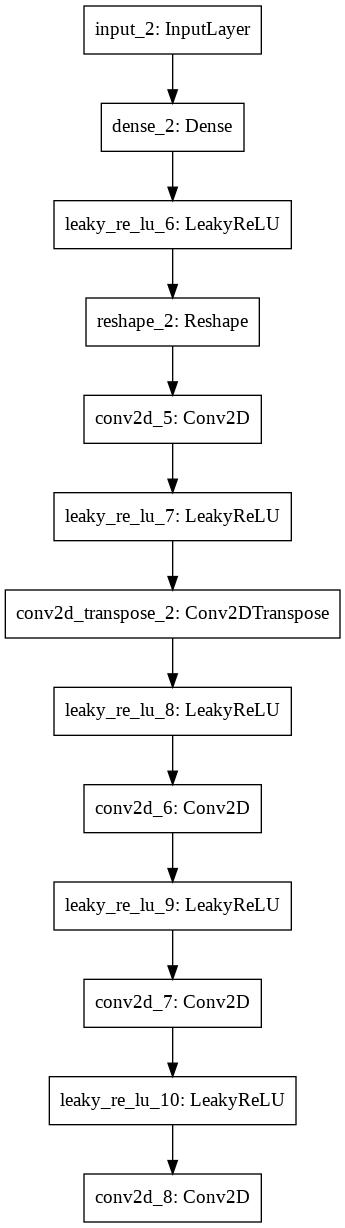
\includegraphics[width=6cm, height=15cm]{Gen.jpeg}
\caption{Our Generator Architecture}
\end{figure}
\begin{figure}[h]
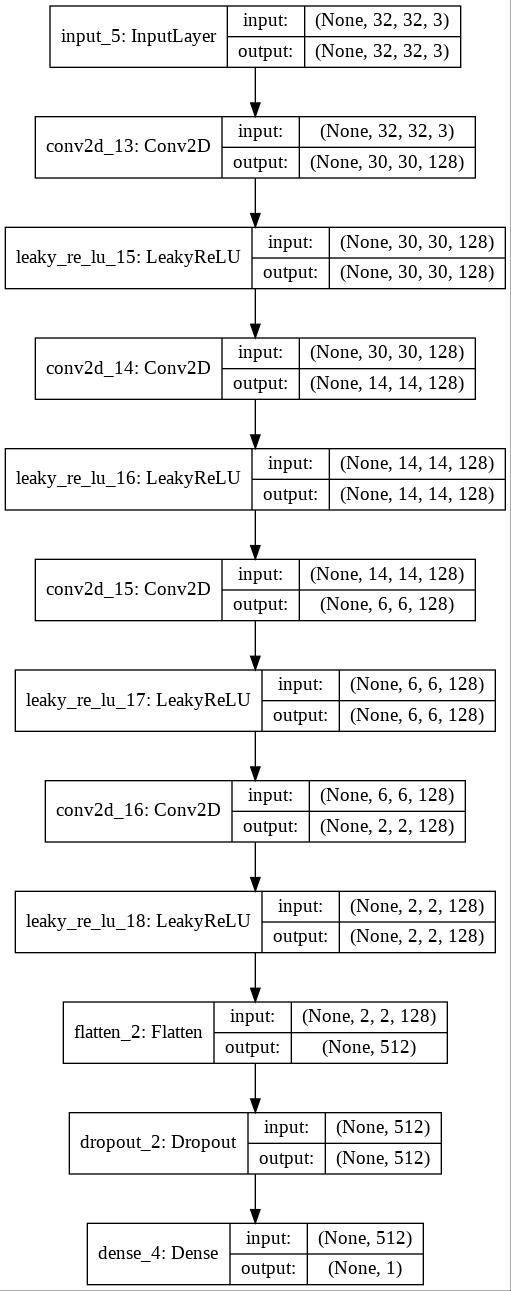
\includegraphics[width=6cm, height=15cm]{Dis.jpeg}
\caption{Our Discriminator Architecture}
\end{figure}
\begin{figure}[h]
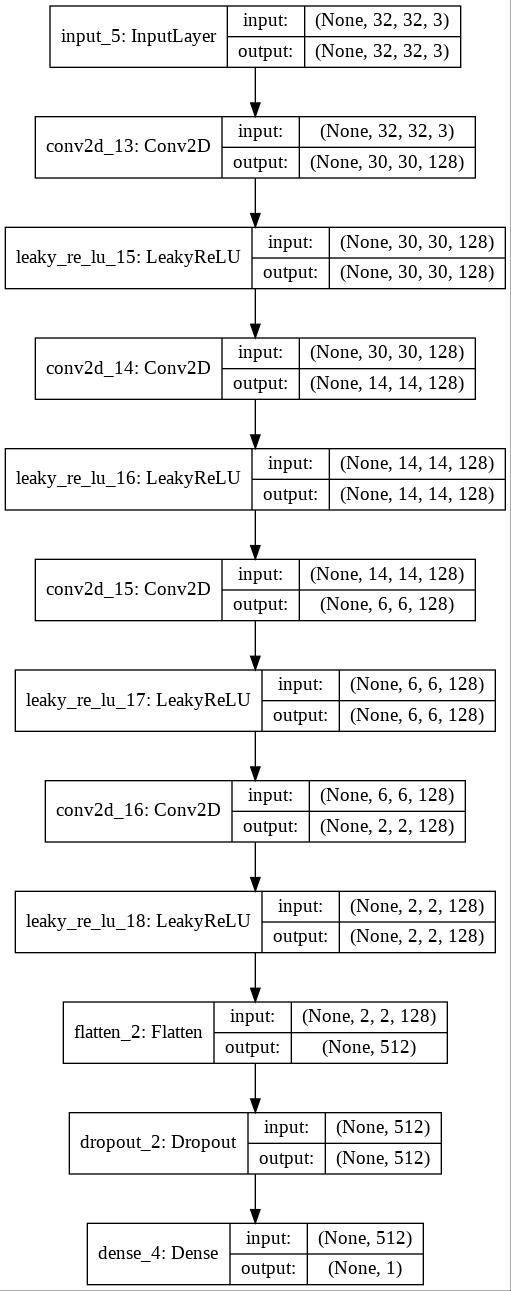
\includegraphics[width=6cm, height=15cm]{GAN.jpeg}
\caption{Our General Adversarial Network Architecture}
\end{figure}
\subsection{Results}
\begin{table}[H]
\centering
\caption{Network Hyperparameters }
\begin{tabular}{|c|c|c|c|c|c|}
\hline
 Iterations & Batch Size & Loss Switch Iteration   \\
\hline
10000 & 20 & 2500 \\
\hline
10000 & 20 & 5000 \\
\hline
10000 & 20 & 7500 \\
\hline
\end{tabular}
\end{table}
\begin{figure}[h]
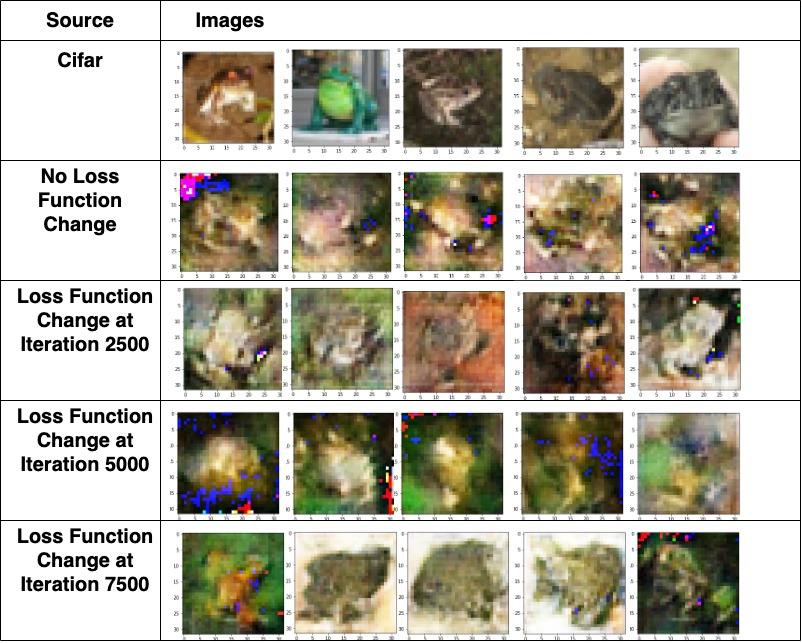
\includegraphics[width=\linewidth]{image_compare.jpg}
\caption{Table Comparing the Results of Various Experiments}
\end{figure}
\section{Conclusion}

\begin{thebibliography}{00}
\bibitem{b1} Goodfellow, I. et al. (2014) Generative Adversarial Networks. arXiv.org. [online]. Available from: http://search.proquest.com/docview/2084531261/
\bibitem{b2} Goodfellow, I. (2016) NIPS 2016 Tutorial: Generative Adversarial Networks.
\bibitem{b3} F. Chollet, “fchollet/deep-learning-with-python-notebooks,” GitHub, 05-Sep-2017. [Online]. Available: https://github.com/fchollet/deep-learning-with-python-notebooks/blob/master/8.5-introduction-to-gans.ipynb. [Accessed: 11-May-2020].
\bibitem{b4} E. Larson, “Generative Networks,” Github, 14-Apr-2020. [Online]. Available: https://github.com/8000net/LectureNotesMaster/blob/master/PDF\_slides/DL\_5\_Generative1.pdf. [Accessed: 10-May-2020].

\end{thebibliography}

\end{document}
